\graphicspath{ {images/3_source_localization/} }
\chapter{Sound Source Localization}
\section{Physical background}
This section introduces the sound propagation model from \cite{physik_skript} which the following described theory is based on.
The sound propagation of an ideal isotropic source follows
\begin{equation}
	I = \frac{P}{4\pi r^2},
\end{equation}
where $I$ is the measurement point, $P$ is the source power and $r$ is the distance
between $I$ and the source.
In this formula the absorption of the air is neglected.
If the sound intensity is measured at two points which are much closer
to each other than they are from the source, the intensities are approximately
$I_1 \approx I_2$.

The propagation speed of sound waves in air is
\begin{equation}
	c = \sqrt{\frac{\aleph R T}{M}}
\end{equation}
with $\aleph$ as the heat capacity ration, R as the gas constant, T as the temperature
and M as the molar mass.
If $c$ is known for a specific temperature $T_0$ the equation is equal to
\begin{equation}
	c(T) = c_{T_0} \sqrt{1 + \frac{T}{T_0}}.
\end{equation}


\section{Sound Source Localization Methods}
\acrfull{ssl} is a well researched area with many applications.
The basic system can be brought into two categories, time based or power based methods.
\subsection{Power based SSL}
The idea of power based SSL is based of the known propagation properties of sound waves in air.
However for this method to work some properties of the sound source have to be known.
Additionally the sensors that measure the sound power levels have to be precise
enough to be able to capture small differences in Sound power levels.
To avoid such demanding hardware requirements this approach was not further
studied in this thesis.

\subsection{Time Based SSL}
Another group of \acrshort*{ssl} is based on the time when the
signal is picked up by the microphones.
Given a source at a location $\bm{S} = (x_S,y_S)^T$ and $N$ microphones at locations
$\bm{M_n} = (x_n,y_n)^T$ the time it takes for a acoustic signal from the source to reach a microphone is
\begin{equation}
	t_n = \frac{\lVert \bm{S} - \bm{M_n}\rVert}{c}
	= \frac{\sqrt{\left(x_S - x_n\right) + \left(y_S - y_n\right)}}{c} .
\end{equation}
So if $t_n$ is known for a microphone, the location of the source can be limited to points on a circle
around $M_n$ with a radius of $t_n c$.
Given three or more microphones, the intersection of these circles will show the location of the source.
However in many cases this approach is not realistic since $t_n$ is generally not known.
It would require some sort of a synchronization between the microphones and the sources.
\subsubsection{Near-Field}
The next time property that could be used is the \acrfull{tdoa} between
two microphones, which is defined as
\begin{equation}
	t_{n, m} = t_m - t_n = \frac{\lVert \bm{S} - \bm{M}_m\rVert - \lVert \bm{S} - \bm{M}_n\rVert}{c}.
\end{equation}
With this equation, $\bm{S}$ can be interpreted as the set of points that lie on a hyperbola
whose fixed points are the Microphones and the vertices are $c t_{n,m}$m apart.
To find the location of $\bm{S}$, a minimum of four microphones is now needed.
This approach only works if we can assume that the curvature of the incoming sound waves
at the microphones is big enough. Figure \ref{ssl:fig:near field} shows such a arrangement,
which is generally known as the near-field scenario.
It is generally said, that the near-field assumption holds when the distance from the source
to the array isn't much greater than the size of the array.
In Figure \ref{ssl:fig:hyperbola}, it can be seen how the resulting hyperbolas from the
\acrshort{tdoa} intersect at the point $\bm{S}$.


\begin{figure}[ht]
	\centering
	\begin{subfigure}[b]{0.45\textwidth}
		\centering
		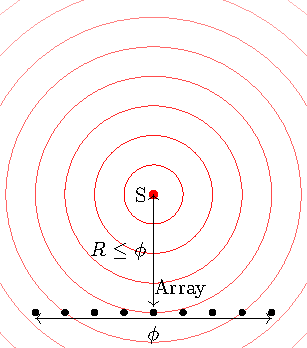
\includegraphics[width=\textwidth]{NearField.pdf}
		\caption{Acoustic model used for the near field \acrshort{ssl}.}
		\label{ssl:fig:near field}
	\end{subfigure}
	\hfill
	\begin{subfigure}[b]{0.45\textwidth}
		\centering
		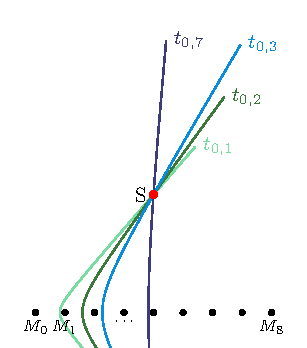
\includegraphics[width=\textwidth]{hyperbola.pdf}
		\caption{A selection of the hyperbolas resulting from the time-delays $t_{m,n}$.}
		\label{ssl:fig:hyperbola}
	\end{subfigure}
	\caption{Near field \acrshort{ssl} with a linear microphone Array.
		Since the microphones are distributed on a straight line a degree of freedom is lost and
		$\bm{S}$ mirrored at this line is also a possible solution.}
	\label{fig:three graphs}
\end{figure}

\subsubsection{Far-Field}
When the source is much further away than the size of the Array, as depicted
in Figure \ref{ssl:fig:far field}, the curvature of the sound wave at the array is negligible.
This is generally known as the far-field case where the sound waves aren't
modeled as spherical waves but rather as planar waves.
Given such a planar wave, only the direction in which the source is placed can be determined with the TDOAs.

% Beamforming_general_S1110865703212038
\begin{figure}[h]
	\centering
	%    \includegraphics[width=0.25\textwidth]{mesh}
	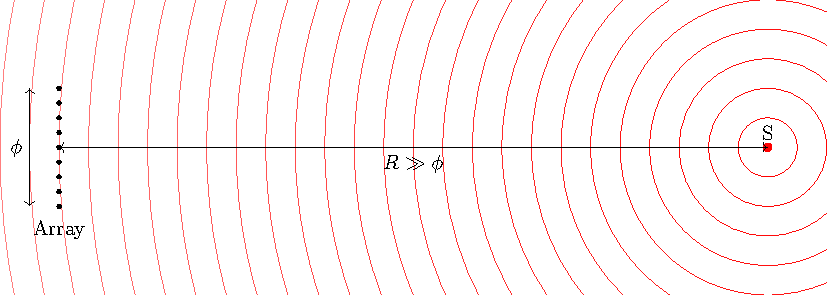
\includegraphics[]{FarField.pdf}
	\caption{Far-Field case. The Curvature of the sound-waves from S at the array
		is almost zero.}
	\label{ssl:fig:far field}
\end{figure}

If the exact localization is required, multiple far field based systems could be
used to triangulate the source position given the calculated direction from each system.

In this thesis the focus was set on far-field techniques considering that the
goal is to detect drones which are usually several meters above ground.
Considering this decision, only the direction in which a sound source is positioned
can be determined with a single system.
\newpage
\subsection{Direction of arrival estimation}
Lots of research has been made on how to estimate the \acrfull*{doa} of a source
with appropriate sensors.
In \cite{s140201918} the authors built a Sound Compass
using MEMS to find the directions of multiple sound sources.
They also followed the approach to use multiple of their devices to
find an exact position of a sound source.
To estimate the \acrshort*{doa} they used a Delay and Sum beamformer,
which is also used in this thesis.

\subsection{Beamforming}
To better show the fundamental principles of beamforming, an example is used
where the goal is not to estimate a \acrshort{doa} but to send a sound wave
in a desired direction using loudspeakers.
Figure \ref{ssl:fig:beamforming1} illustrates such a case in $\mathbb{R}^2$,
where a linear array of N sound sources beam a sine wave $x(t) = \sin(\omega_0 t)$
in the direction of $\varphi$.
This is achieved by adding a phase shift to the sine wave
at each microphone, resulting in $x_n(t) = sin(\omega_0 t - \omega_0t_n)$.
If the phase shifts are properly selected the points where the waves positively
interfere form a beam.
Using this example with a narrow band signal, the output at each source
can be written as
\begin{equation}
	x_n(t) = \Re(sin(\omega_0 t) e^{-j\omega t_n})
\end{equation}
and more generalized as
\begin{equation}
	\label{ssl:eq:beamSteerOut}
	\bm{X}(t, \varphi) =
	\Re\left(
	sin(\omega_0 t)
	\underbrace{
		\begin{pmatrix}
			e^{-j\omega_0 t_0(\varphi)} \\
			e^{-j\omega_0 t_1(\varphi)} \\
			\vdots                      \\
			e^{-j\omega_0 t_{N-1}(\varphi)}
		\end{pmatrix}}_{\bm{W}(\varphi)}
	\right).
\end{equation}
The vector $\bm{W}(\varphi)$ is commonly known as the steering vector.
It can be seen that the steering vector is dependent on $\omega_0$ and
will therefore only have the desired effect on signals with frequencies
close to $\omega_0$.
The idea will be expanded to wide band signals later in this chapter.
\begin{figure}
	\centering
	%    \includegraphics[width=0.25\textwidth]{mesh}
	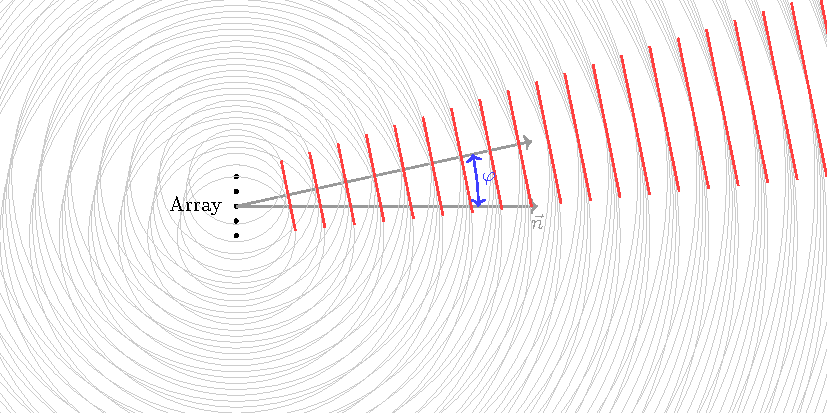
\includegraphics[]{beamforming_1.pdf}
	\caption{Phase differences between the array elements create positive interference at the red lines.
		The gray circles correspond the waves' local maxima}
	\label{ssl:fig:beamforming1}
\end{figure}

If the goal is to estimate the direction of a sound signal with microphones
$x_n(t)$ is redefined as the signal measured by the $n$th microphone.
Now \eqref{ssl:eq:beamSteerOut} is rewritten to
\begin{equation}
	\label{ssl:eq:beamSteerIn}
	\bm{Y}(t, \varphi) =
	\underbrace{
		\begin{pmatrix}
			x_0(t) \\
			x_1(t) \\
			\vdots \\
			x_{N-1}(t)
		\end{pmatrix}}_{\bm{X}(t)}
	\odot
	\underbrace{
		\begin{pmatrix}
			e^{-j\omega_0 t_0(\varphi)} \\
			e^{-j\omega_0 t_1(\varphi)} \\
			\vdots                      \\
			e^{-j\omega_0 t_{N-1}(\varphi)}
		\end{pmatrix}}_{\bm{W}(\varphi)}
\end{equation}
where depending on the beamforming method used either $\bm{Y}(t, \varphi)$ is further processed, or the
method directly uses $\bm{X}(t)$ for the \acrshort*{doa} estimation.

\subsubsection{Steering Vector}
The calculation of the Steering Vector is dependent on different factors.
The two main factors can be broken down to the geometry of the microphone array
and the direction in which the source lies.
Again the formulas are derived for a circular array in $\mathbb{R}^2$ and are then expanded into $\mathbb{R}^3$.
A circular array where all the microphones are
placed on a circle is used for the derivation, the theory can however
be expanded to any array geometry in $\mathbb{R}^2$.

Figure \ref*{ssl:fig:steering} shows a circular array with five equally spaced microphones $M_n$.
The goal of the steering vector is to delay the measured signal at each microphone, so that
they have the same phase and therefore positively interfere.
To calculate these delays a reference point must first be defined.
Here it is the center of the circle.
With the far field model, the sound pressure level is equal along lines perpendicular
to its propagation direction.
Therefore the magenta line is the reference line and each measured signal from the microphones must be
phase shifted with
\begin{equation}
	\omega_0 t_n =
	\omega_0 \frac{
		\bm{d}_n(\varphi_s) \cdot \hat{\bm{d}}_s}
	{c}.
\end{equation}
Simplifying this equation with
\begin{equation}
	\bm{d}_n(\varphi_s) \cdot \hat{\bm{d}}_s = r_{m_n} \cos(\varphi_s - \varphi_{m_n})
\end{equation}
results in
\begin{equation}
	t_n(\phi_s) =
	r_{m_n} \cos(\varphi_s - \varphi_{m_n})
	\frac{1}{c}.
	\label{ssl:eq:beamr2}
\end{equation}
This formula can be used for any microphone with polar coordinates
$(\varphi_{m_n}, r_{m_n})$ and can therefore be used for any array configuration
described in polar coordinates.

\begin{figure}[h]
	\centering
	%    \includegraphics[width=0.25\textwidth]{mesh}
	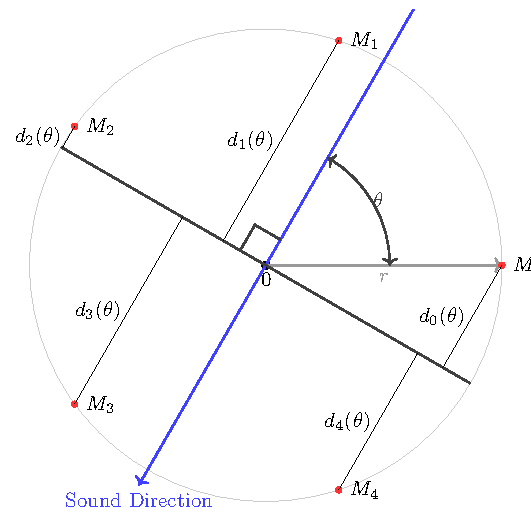
\includegraphics[]{steering_vector.pdf}
	\caption{Distances between each microphone and the reference line in
		a circualr microphone array.}
	\label{ssl:fig:steering}
\end{figure}


To expand this idea into $\mathbb{R}^3$ the spherical coordinate system is used.
This adds the angle $\theta$ as the inclination.
When $\theta = \pi/2$ it is the same situation as with the polar coordinate system.
As $\theta$ approaches 0 the speed of the wavefront projected onto the
surface of the array increases, until the sound wave reaches every microphone
simultaneously when $\theta = 0$.
This expands \eqref{ssl:eq:beamr2} to
\begin{equation}
	t_n(\phi_s, \theta_s) =
	r_{m_n} \cos(\varphi_s - \varphi_{m_n})
	\frac{\sin(\theta_s)}{c}.
	\label{ssl:eq:beamr3}
\end{equation}
To simplify the formulas, $t_n(\phi, \theta)$ is from now on written as $t_n$.

\subsubsection{Delay and Sum Beamformer}
The basic beamforming is the delay and sum beamforming
\begin{equation}
	\label{ssl:eq:delAndSum}
	y(t, \varphi, \theta) =
	\underbrace{
		\begin{pmatrix}
			x_0(t) \\
			x_1(t) \\
			\vdots \\
			x_{N-1}(t)
		\end{pmatrix}}_{\bm{X}(t)}
	\cdot
	\underbrace{
		\begin{pmatrix}
			e^{-j\omega_0 t_0(\varphi, \theta)} \\
			e^{-j\omega_0 t_1(\varphi, \theta)} \\
			\vdots                              \\
			e^{-j\omega_0 t_{N-1}(\varphi, \theta)}
		\end{pmatrix}}_{\bm{W}(\varphi, \theta)}.
\end{equation}
Notice how instead of the Hadamard product, the scalar product is now used resulting
in $y(t, \varphi, \theta)$ as the sum of the delayed signals.
If the angles of the steering vector point towards a source its
signal will be amplified.

Beamforming can be visualized with the so called beam pattern.
It shows how much a sound of a source at a specific location
is amplified depending on the steering direction.
By using the delays calculated for the steering vector $\bm{X}(t)$ can
be calculated to simulate a source in a specific direction
\begin{equation}
	\bm{X}(t, \varphi_s, \theta_s) =
	e^{j\omega_0 t}
	\begin{pmatrix}
		e^{j\omega_0 t_0(\varphi_s, \theta_s)} \\
		e^{j\omega_0 t_1(\varphi_s, \theta_s)} \\
		\vdots                                 \\
		e^{j\omega_0 t_{N-1}(\varphi_s, \theta_s)}
	\end{pmatrix}
\end{equation}

The response of an array using delay and sum beamforming can
now be calculated with
\begin{equation}
	G(\phi, \theta) =
	\frac{
		\lvert X(0, \phi_s, \theta_s) \cdot W(\phi, \theta) \rvert}
	{
		N
	}.
\end{equation}
The response is normalized with the amount of microphones to ensure a maximum
gain of 1.
In Figure \ref*{ssl:fig:CircBmResponse} two such responses with can be seen.
The main lobe of $G(\phi, \theta)$ clearly shows in the direction of the source
however there are also side lobes pointing to directions without sources.

\begin{figure}[ht]
	\centering
	\begin{subfigure}[t]{0.45\textwidth}
		\centering
		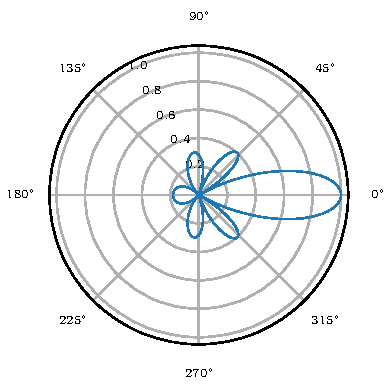
\includegraphics[width=\textwidth]{radial_1200_circ_single.pdf}
		\caption{\(G(\phi, \theta, \omega)\) with $\theta = \pi/2$ for $\omega_0 = 2\pi 1000$.
			The source is placed in the direction of $(\phi=0, \theta = \pi/2)$}
		\label{ssl:fig:CircBmPhi}
	\end{subfigure}
	\hfill
	\begin{subfigure}[t]{0.45\textwidth}
		\centering
		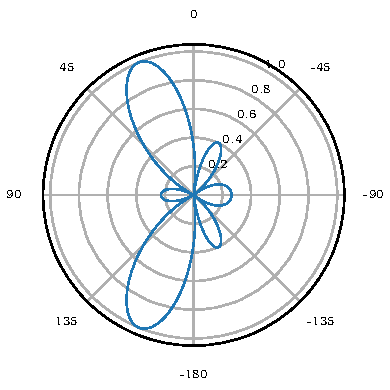
\includegraphics[width=\textwidth]{radial_1200_circ_theta_single.pdf}
		\caption{\(G(\phi, \theta, \omega)\) with $\phi = 0$ for for $\omega_0 = 2\pi 1000$.
			$(\phi= 0, \theta = -45^\circ)$ is the same as $(\phi= 180^\circ, \theta = 45^\circ)$.
			The mirror along the horizontal axis comes from the flat geometry of the array which makes
			it impossible to distinguish if a sound comes from $\theta$ or $180 + \theta$.}
		\label{ssl:fig:CircBmTheta}
	\end{subfigure}
	\caption{Beam patterns of delay and sum beamforming using a circular array with $N=16$ microphones
		and a radius $r = 0.25$m. Note that the gains are applied on the amplitudes, so the
		power levels are multiplied by $G(\dots)^2$}
	\label{ssl:fig:CircBmResponse}
\end{figure}

\subsubsection*{Wide band delay and sum beamforming}
Until now the formulas are only useful for narrow band signals.
This theory is now expanded to be applicable for wide band signals.

The narrow band delay and sum beamforming has the property, that it behaves
the same in the frequency domain
\begin{equation}
	e^{-j\omega_0 t_n} x_n(t) = \mathscr{F}^{-1}(e^{-j\omega_0 t_n} \mathscr{F}(x_n(t)))
\end{equation}
since it is just a multiplication with a scalar,.
The summation could also be done in the frequency domain due to the
linearity of the Fourier transform.
The frequency domain has the advantage that an IIR Filter can be constructed, to
make a different phase shift for every frequency
\begin{equation}
	\label[type]{ssl:eq:iirbeam1}
	Y_n(t) = \mathscr{F}^{-1}(e^{-j\omega t_n} X_n(\omega)).
\end{equation}
By using a discrete fourier transform the beamformer can be written
in matrix form
\begin{equation}
	\bm{Y}(\phi, \theta) =
	\begin{pmatrix}
		X_0(\omega_l)     & \hdots & X_0(\omega_h)     \\
		\vdots            & \ddots & \vdots            \\
		X_{N-1}(\omega_l) & \hdots & X_{N-1}(\omega_h)
	\end{pmatrix}
	\odot
	\begin{pmatrix}
		e^{-j\omega_l t_0}     & \hdots & e^{-j\omega_h t_0}     \\
		\vdots                 & \ddots & \vdots                 \\
		e^{-j\omega_l t_{N-1}} & \hdots & e^{-j\omega_h t_{N-1}}
	\end{pmatrix},
\end{equation}
with a total of $M$ frequency points of interest between $\omega_l$ and $\omega_h$.
The power of the signal is now calculated with
\begin{equation}
	P(\phi, \theta) =  \sum_{m=0}^{M-1}\lvert \sum_{n=0}^{N-1} \bm{Y}_{m, n} \rvert^2
\end{equation}
using Parsevals' Theorem.
This beamformer does not need to be implemented in the frequency domain.
Delaying each signal in the time domain is equivalent.

\subsubsection{Spatial Sampling}
\label{sec:spatSam}
Beamforming can be seen as spatial sampling, where the microphones
are the samplingpoints.
So some of the concepts used in digital sampling such as
the samplingtheorem and the uncertainty principle can also
occur in some way in beamforming.
Figure \ref{ssl:fig:f_deps} shows the beam pattern for different frequencies.
The array used in Figure \ref{ssl:fig:f_dep0} is the same array
as in Figure \ref*{ssl:fig:CircBmResponse} whereas Figure \ref{ssl:fig:f_dep0}
uses a circular array with $r = 0.5$m and also 16 microphones.
It can be seen that at around 1500hz more side lobes with a
high amplitude start to appear.
With this array geometry the smallest distance between two
microphones is $\approx 0.098$m, which is the wavelength
of a sound wave with a frequency of approximately 3500hz.
So the effect seen in Figure \ref*{ssl:fig:CircBmResponse} is
a kind of aliasing.
This results from ambiguity in the phases of the steering vector.
Ideally the phase shift between two neighboring microphones is unique
for each angle of the steering vector.
However when they are more than $\lambda/2$ apart, phase shifts start to
repeat for different steering directions.

Another effect seen in Figure \ref*{ssl:fig:f_dep0} is the increase
of the main lobe width when the frequency approaches 0.
This is consequence of a too small array.
In the used array the maximal distance between two microphones is 0.5m.
For lower frequencies the phase difference between the first microphone and
the last microphone in the array is too small to get destructive
interferences when the steering vector is not focused on the source.
As expected the bigger array from Figure \ref*{ssl:fig:f_dep1} has a smaller
main lobe in the lower frequencies.

\begin{figure}[h]
	\centering
	\begin{subfigure}[t]{0.45\textwidth}
		\centering
		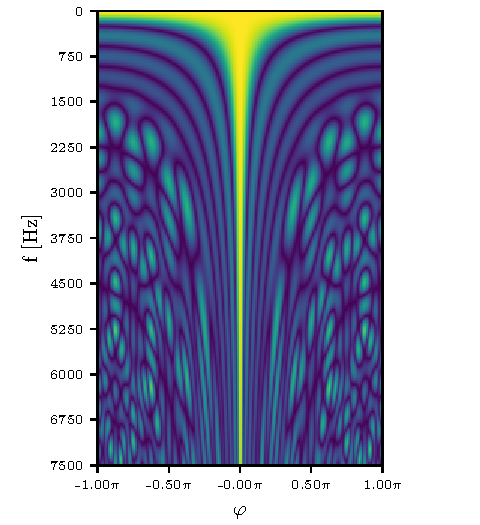
\includegraphics[width=\textwidth]{circ_f_sweep_0.pdf}
		\caption{$G(0, 90^\circ)$ for a circular array with a radius of 0.25m.}
		\label{ssl:fig:f_dep0}
	\end{subfigure}
	\hfill
	\begin{subfigure}[t]{0.45\textwidth}
		\centering
		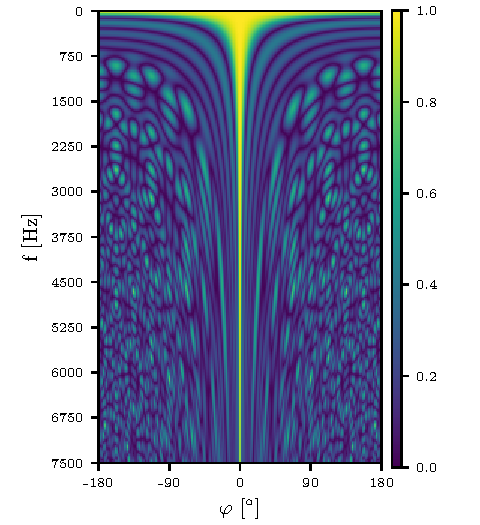
\includegraphics[width=\textwidth]{circ_f_sweep_1.pdf}
		\caption{$G(0, 90^\circ)$ for a circular array with a radius of 0.5m.}
		\label{ssl:fig:f_dep1}
	\end{subfigure}
	\caption{Delay and Sum Beamformer response for two circular arrays with $N=16$ microphones
		and a radiuses of 0.25m an 0.5m. }
	\label{ssl:fig:f_deps}
\end{figure}
\section{Tracking}
By now the \acrshort{doa} of a sound source can be estimated.
But since drones expected to be moving, a source once it has been
detected, needs to be tracked.

In \cite{GuiAhmad} the tracking is done with by
updating the steering vector with an adaptive filter.
They however do not go into detail on how the direction is then
retrieved from the steering vector.
One possibility may be by looking at the $G(\phi, \theta)$ of the steering vector.
But what makes this definitely not used in this thesis, is that its based on a
narrow band beamformer.
Developing a beamforming based tracker for a wide band beamformer was outside of the
scope of this thesis.

Another popular object tracker independent of beamforing is a Kalman filter based tracker.
It takes a measured position as an input and calculates the estimated position with
a Kalman filter.
The basic model for the Kalman filter is, that the source moves with a constant velocity leading to
the state and observation matrix
\begin{equation*}
	\bm{x}(n) =
	\begin{pmatrix}
		x_n       \\
		y_n       \\
		z_n       \\
		\dot{x}_n \\
		\dot{y}_n \\
		\dot{z}_n \\
	\end{pmatrix},
	\bm{A}(n) =
	\begin{pmatrix}
		1 & 0 & 0 & \Delta T & 0        & 0        \\
		0 & 1 & 0 & 0        & \Delta T & 0        \\
		0 & 0 & 1 & 0        & 0        & \Delta T \\
		0 & 0 & 0 & 1        & 0        & 0        \\
		0 & 0 & 0 & 0        & 1        & 0        \\
		0 & 0 & 0 & 0        & 0        & 1        \\
	\end{pmatrix},
	\bm{C}(n) =
	\begin{pmatrix}
		1 & 0 & 0 & 0 & 0 & 0 \\
		0 & 1 & 0 & 0 & 0 & 0 \\
		0 & 0 & 1 & 0 & 0 & 0 \\
	\end{pmatrix}
\end{equation*}
The velocity in the state vector also enables blind prediction.

To enable multi object tracking, another processing step is added.
First the new measured objects are assigned to the already
existing trackers.
To make this assignment somehow optimal, the Hungarian algorithm
with the measurement and blind prediction of each Kalman filter as input, is used.
If the distance between the prediction and measured object position of a pair is close enough
the Kalman filter is run with the measured position as input.
However if they are far apart, the measured object is treated as a new object
and is assigned to a new Kalman filter instance.

Note that the tracker is in the cartesian coordinate system.
The transformation from a \acrshort*{doa} to a cartesian point is
covered in Section \ref*{chap:fin:sw}

\newpage
\section{Simulator}
In order to experiment with different microphone arrangements and algorithms a simulator in Python was developed.
Since the simulator wasn't the main focus of this Thesis, its functionality was kept simple.
The simulator lets you place acoustic sources and microphones in a $\mathbb{R}^3$ space and calculates
the measured signals at each microphone.

\subsection{Simulation Model}
For sake of simplicity the sources were modeled as omnidirectional point-sources and the
microphones are omnidirectional as well.
The Sound Pressure Level of a source is defined at one meter distance from their position and decreases
squarely with the distance.
The perceived sound at any point $P$ can now be described as
\begin{equation}
	\label[type]{ssl:eq:simcont}
	y(P, t) = \sum_{I} \frac{x_i(t - \lVert P - S_i\rVert/c)}{\lVert P - S_i\rVert}.
\end{equation}
Where $S_i$ is the position of the nth Source and $x_i(t)$ is its output sound.
Since the simulation is done numerically and with pre recorded audio files with a given
samplingrate $f_s$ \eqref{ssl:eq:simcont} has to be discretized.
Simply replacing
\begin{equation*}
	x_i(t - \lVert P - S_i\rVert/c)
\end{equation*}
with
\begin{equation*}
	x_i(t_n - f_s \lVert P - S_i\rVert/c),
\end{equation*}
with
\begin{equation*}
	t_n = t_0 + n f_s, n \in \mathbb{N}
\end{equation*}
doesn't work because
$f_s \lVert P - S_i\rVert/c \not \in \mathbb{N}$ in most cases.
To implement this $f_s \lVert P - S_i\rVert/c$ is rounded to
its nearest integer $d_{P,S_i}$.
Now the delayed signal is $x_i(t_n - d_{P,S_i})$.
To achieve sub sample delays this signal is then filtered
with a Fractional Delay FIR Filter \cite{FracFil} with a delay of
$f_s \lVert P - S_i\rVert/c - d_{P,S_i}$.

\subsubsection{Reflections}
The simulator also allows the reflective surfaces to be placed into the room.
These surfaces are defined with a base vector and two directional vectors and have a infinite size.
Additionally a dampening factor can be defined which defines how much
a reflecting sound signal is damped when getting reflected.
By this stage the simulator can only handle single reflective path.
An already reflected sound signal can not be reflected by a second surface.

\subsection{Output}
The simulator saves WAV files for each microphone, with the audio signal from
each source as a single chanel.
It can also be installed as a python package with its Github link.
In this case, the simulator can also return the recorded signals as an
Numpy array.
